\documentclass{report}
\usepackage[T1]{fontenc}
\usepackage[utf8]{inputenc}
\usepackage{lmodern}
%\usepackage{hyperref}
\usepackage[portuges,brazilian]{babel}
\usepackage{graphicx}
\usepackage{textcomp}
\usepackage{fullpage}
\usepackage{wrapfig}
\usepackage{float}
\usepackage{listings}
\usepackage{amsmath}
\usepackage{amssymb}
\usepackage{subcaption}
\begin{document}

\newcommand{\HRule}{\rule{\linewidth}{0.5mm}}
\newcommand{\tsize}[1]{(\frac{W}{L})_{#1}}
 

%%%%%%%%%%%%%%%%%%%%%%%%%% START TITLE PAGE %%%%%%%%%%%%%%%%%%%%%%%%5
\begin{titlepage}

\begin{center}


{\LARGE UNIVERSIDADE DE SÃO PAULO\\}
{\LARGE DEPARTAMENTO DE ENGENHARIA ELÉTRICA \\}
{\LARGE ESCOLA DE ENGENHARIA DE SÃO CARLOS\\[4cm]}

\textbf{\large SEL5755 - Sistemas Fuzzy}\\[1cm]
\textbf{\large Prof Dr. Ivan Nunes da Silva}\\[2cm]


% Title
\HRule \\[0.6cm]
{ \huge EPC 6\bfseries }\\[0.6cm]

\HRule \\[2cm]

% Author

\begin{center} \large
\emph{Alunos:}\\
\end{center}

\begin{minipage}{0.4\textwidth}
\begin{flushleft} \large
Isabela R. do Prado \textsc{Rossales}\\
6445435
\end{flushleft}
\end{minipage}
\begin{minipage}{0.4\textwidth}
\begin{flushright} \large
Jonas Rossi \textsc{Dourado}\\
6445442
\end{flushright}
\end{minipage}

\vfill

% Bottom of the page
{\large São Carlos,\\ \today}

\end{center}

\end{titlepage}
%\listoffigures
%\begingroup
%\let\clearpage\relax
%\listoftables
%\endgroup
%%%%%%%%%%%%%%%%%%%%%%%%%% STOP TITLE PAGE %%%%%%%%%%%%%%%%%%%%%%%%5


\newpage

Para um sistema elétrico de potência, representado na Figura 1, há a necessidade de
se classificar distúrbios relacionados à qualidade da energia elétrica.

\begin{figure}[hptb]
\centering
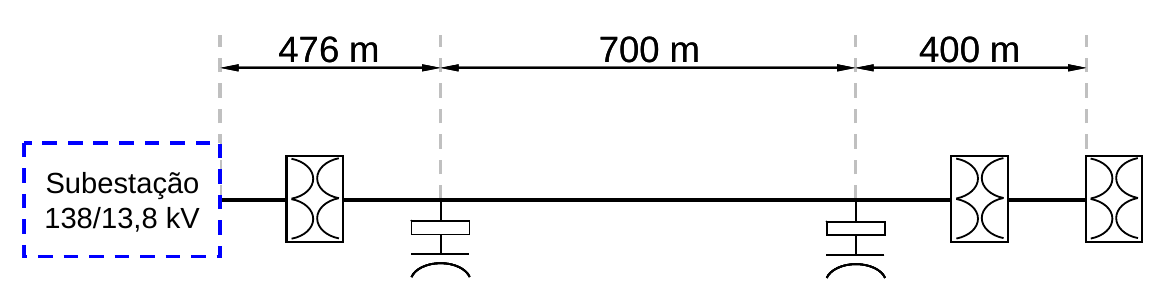
\includegraphics[scale=.6]{diagrama.png}
\label{diagrama}
\caption{Diagrama do sistema de potência.}
\end{figure}

Assim, baseado em medições de grandezas elétricas, pretende-se projetar um sistema
fuzzy de tipo Mamdani para classificar os seguintes tipos de distúrbios:

\begin{enumerate}
 \item Interrupção
 \item Afundamento
 \item Elevação
 \item Operação Normal
 \item Presença de Harmônicas
\end{enumerate}

A ilustração do sistema fuzzy é mostrada na Figura \ref{esquematico}, cujas variáveis de entrada são a
tensão fundamental ($V_f$) em p.u. (per unit) e a distorção harmônica total (DHT) em \%.

\begin{figure}[hptb]
\centering
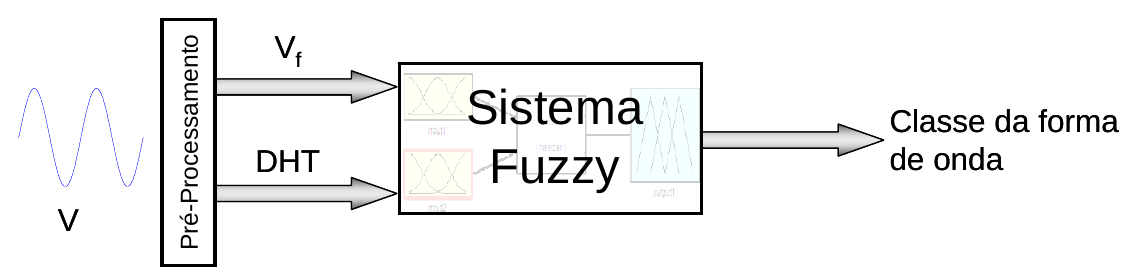
\includegraphics[scale=.6]{esquematico.png}
\label{esquematico}
\caption{Diagrama esquemático do sistema fuzzy.}
\end{figure}

Implemente então um sistema fuzzy do tipo Mamdani com as seguintes características:

\begin{enumerate}
 \item Utilizar 200 pontos de discretização para todos os universos de discurso.
 \item Utilizar operador de composição do tipo Max-Min.
 \item Utilizar como operador de implicação o operador de Mamdani.
 \item Utilizar como operador de agregação o operador Máximo.
 \item Utilizar o operador Mínimo para o conectivo “e”.
\end{enumerate}

As especificações das variáveis de entradas e saída são definidas conforme se segue.

\section{Entrada 1: Tensão Fundamental ($V_f$)}

Variável lingüística: Vf (pu)

Termos Lingüísticos: “Muito Baixa”, “Baixa”, “Média” e “Alta”

Funções de Pertinência: “Trapezoidal”

Universo de discurso: [0;1,8] (p.u.)


\begin{center}
\begin{tabular}{lllll}
Termo Lingüístico & a & m & n & b\\
Muito Baixa & 0.00 & 0.00 & 0.09 & 0.12\\
Baixa & 0.09 & 0.12 & 0.94 & 0.96\\
Média & 0.94 & 0.96 & 1.04 & 1.06\\
Alta & 1.04 & 1.10 & 1.80 & 1.80\\
\end{tabular}
\end{center}



\section{Entrada 2: Distorção Harmônica Total em \% (DHT)}

 Variável linguística: DHT (\%)

 Termos Linguísticos: “Pequena”, “Grande”

 Funções de Pertinência: “Trapezoidal”

 Universo de discurso: [0;100] (\%)


\begin{center}
\begin{tabular}{lllll}
Termo Linguístico & a & m & n & b\\
Pequena & 0 & 0 & 5 & 6\\
Grande & 5 & 7 & 100 & 100
\end{tabular}
\end{center}



\section{Saída: Classe da Forma de Onda}

Variável lingüística: Classe

Termos Lingüísticos: “Interrupção”, “Afundamento”, “Elevação”, “Operação Normal”, “Presença de Harmônicas”

Funções de Pertinência: “Triangulares”

Universo de discurso: [0 1] (normalizado)


\begin{center}
\begin{tabular}{llll}
Termo Lingüístico & a & m & b\\
Interrupção & 0.000 & 0.167 & 0.333\\
Afundamento & 0.167 & 0.333 & 0.500\\
Operação Normal & 0.333 & 0.5 & 0.667\\
Elevação & 0.500 & 0.667 & 0.833\\
Harmônicas & 0.667 & 0.833 & 1.000
\end{tabular}
\end{center}

O conjunto de regras é especificado em função das seguintes sentenças lingüísticas:\\
Regra 1 -> Se Vf é Muito Baixa e DHT é Pequena então Saída é Interrupção.\\
Regra 2 -> Se Vf é Baixa e DHT é Pequena então Saída é Afundamento.\\
Regra 3 -> Se Vf é Média e DHT é Pequena então Saída é Operação Normal.\\
Regra 4 -> Se Vf é Alta e DHT é Pequena então Saída é Elevação.\\
Regra 5 -> Se Vf é Muito Baixa e DHT é Grande então Saída é Interrupção.\\
Regra 6 -> Se Vf é Baixa e DHT é Grande então Saída é Harmônicos.\\
Regra 7 -> Se Vf é Média e DHT é Grande então Saída é Harmônicos.\\
Regra 8 -> Se  Vf é Alta e  DHT é Grande então Saída é Harmônicos.\\

Como estratégia para definição de classes, utilize então as seguintes faixas:

\begin{figure}[hptb]
\centering
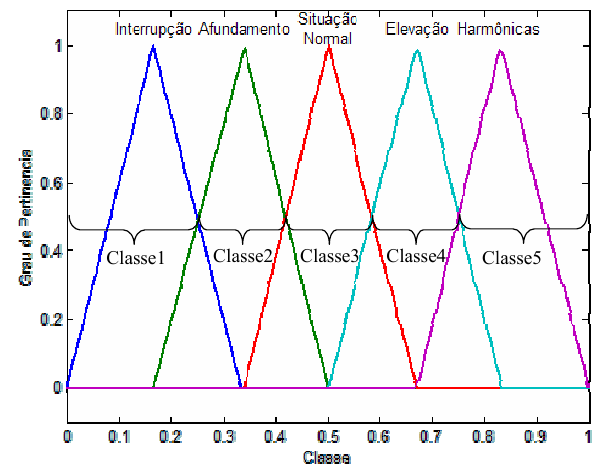
\includegraphics[scale=.6]{classe.png}
\label{esquematico}
\caption{Classes de saída}
\end{figure}


\begin{center}
\begin{tabular}{ll}
Fenômeno & Saída (y)\\
Classe 1 – Interrupção & 0.00 < y $\leq$ 0.25 \\
Classe 2 – Afundamento & 0.25 < y $\leq$ 0.42 \\
Classe 3 – Operação Normal & 0.42 < y $\leq$ 0.58 \\
Classe 4 – Elevação & 0.58 < y $\leq$ 0.75 \\
Classe 5 – Harmônicas & 0.75 < y $\leq$ 1.00
\end{tabular}
\end{center}




Após a implementação de todo o sistema fuzzy, aplique-o então para classificar as
seguintes situações:


\begin{center}
\begin{tabular}{llll}
Situação & $V_f$(pu) & DHT(\%) & Fenômeno \\
1 & 0.01 & 0.34 & \\
2 & 0.05 & 16.26 & \\
3 & 0.50 & 4.84 & \\
4 & 0.85 & 1.79 & \\
5 & 1.02 & 0.47 & \\
6 & 0.97 & 1.21 & \\
7 & 1.57 & 4.76 & \\
8 & 1.26 & 1.21 & \\
9 & 0.99 & 16.32 & \\
10 & 1.20 & 18.96 &
\end{tabular}
\end{center}


\newpage
% \lstinputlisting[language=Python]{ex1.py}

\end{document}
